\documentclass[pdftex,12pt]{article}
\usepackage[pdftex]{graphicx,color}
\usepackage{setspace}
\usepackage{amsmath,amssymb}
\usepackage{titlesec}
\usepackage{subfigure}
\usepackage{fancyhdr}
\usepackage[longnamesfirst]{natbib}
\usepackage{cite}
\usepackage[paperwidth=8.5in,
left=0.75in,right=0.75in,paperheight=11.0in,textheight=9.50in]{geometry}
\usepackage{xcolor}
\usepackage{booktabs}

\bibliographystyle{ecta}


\definecolor{nblue}{RGB}{0,0,128}

\usepackage[pdftex,bookmarks=false,
pdfdisplaydoctitle = {true},
pdfstartview={XYZ null null 0.65},
pdftitle={CEMFI NOTES: The Distributional Consequences of Trade and Policy Responses.},
pdfauthor={Michael E. Waugh},
pdfkeywords={economics, trade, dynamics, quant econ, consumption, data science, cars, waugh, incomplete markets, inequality, Ricardo, julia, migration, China, trade war, tariffs },
colorlinks=true,linkcolor=darkgray,citecolor=darkgray,urlcolor=darkgray,
breaklinks]{hyperref}


\usepackage{setspace}

\onehalfspace

\renewcommand{\baselinestretch}{1.15}
\renewcommand{\arraystretch}{.7}
\setlength{\parindent}{0em}
\setlength{\parskip}{.1in}
\renewcommand\familydefault{\sfdefault}

\titleformat{\section}{\large\bf}{\thesection.}{.5em}{}
\titleformat{\subsection}{\normalsize\bf}{\thesubsection.}{.5em}{}
\titleformat{\subsubsection}{\normalsize\bf}{\thesubsubsection.}{.5em}{}

\def\thesection{\arabic{section}}
\def\thesubsection{\Alph{subsection}}
\def\thesubsubsection{\Roman{subsubsection}}

\newtheorem{proposition}{Proposition}

\newtheorem{as}{Assumption}
\newtheorem{reg}{Regularity Condition}
\newtheorem{conjecture}{Conjecture}
\newtheorem{corr}{Corollary}
\newtheorem{df}{Definition}
\newtheorem{lemma}{Lemma}
\newtheorem{prp}{Proposition}
\newtheorem{rmk}{Remark}
\newenvironment{prf}{{\bf Proof}}{\hfill { }}

\DeclareMathOperator*{\plim}{plim}
\DeclareMathOperator*{\umax}{max}

%\pagestyle{empty}
\lhead{}
\rhead{}
\rfoot{\date}
\cfoot{\thepage}
\lfoot{}
\renewcommand{\headrulewidth}{0pt}

\def\citeapos#1{\citeauthor{#1}'s (\citeyear{#1})}

\lfoot{Revised:  \today}

\begin{document}

\pagestyle{fancy}

\noindent \textbf{\href{http://www.waugheconomics.com/}{\large Measuring Trade Elasticities}}\\
\noindent \textbf{\href{http://www.waugheconomics.com/}{Michael E. Waugh}}\\


If trade policy changes, how will trade flows change? What are the gains from trade associated with the change in policy? These are, perhaps, the central questions of the field of international trade. And they are questions that are of immediate importance given the changes in US trade policy over the last several years.

Ok, so how do we answer these questions. How can we predict, understand, and arrive at normative conclusions with respect to changes in trade policy. While there are many ways to approach this question, what we do know is that a key input into any answer is how elastic trade flows are to changes in trade frictions (broadly defined). The idea (Ian's idea actually) behind these notes are to provide my perspective on measuring this elasticity.

I'm going to do several things. I'll provide an overview as to why we know this is so important. And in this context, I discuss two approaches to measuring the trade elasticity. The first is the a ``price gap'' approach which was first pioneered by \citet{eaton2002technology} and then refined in my work with \citet{sw_jie} and \citet{simonovska2014trade}. This approach will be contrasted with the approach advocated by \citet{arkolakis2012new} and used in \citet{caliendo2014estimates} (as just an example) which uses direct, observable measures of trade policy to estimate trade elasticities.

Both approaches are useful. But both take very different approaches to what is in the unobservable component in the ``gravity regression.'' And it's this issue, how to we think about the unobservable component, which is the key issue when thinking about measuring the trade elasticity. In \citet{sw_jie} and \citet{simonovska2014trade} we think about the unobservable component through the lens of particular model, then use restrictions imposed by theory on the unobserved component to estimate the trade elasticity.  In the approach advocated by \citet{arkolakis2012new}, direct assumptions on the unobservable component are made to facilitate estimation, with the benefit of not having to take a stand on the particular trade model.

With this contrast highlighted, one of the remarkable successes is that these approaches do give similar estimates. This is a lot of progress since the survey of \citet{anderson2004trade} which essentially said, we don't know much, but what we know is within the range of 5-10.

Finally, I'll discuss some of these issues in the context of the current US-China trade war and things that I have found in \citet{waugh_consumption}. While the trade war is unprecedented, how trade flows are responding is not. In fact, a lot of what I'm finding lines up very well with the estimates that arise out of the alternative approaches discussed above.

\section{What is the issue?}
What is remarkable about how much synthesis has occurred in the trade literature regarding some issues. A lot of this foundation was all set up in \citet{arkolakis2012new} with what are essentially several statements about ``applied general equilibrium trade models.'' I'm going to formulate it in this way:

\textbf{Claim \#1.} Fix a particular model trade model of your favorite variety. We will get something like
\begin{enumerate}
\item This model has a ``gravity representation'' which takes the form like this
\begin{eqnarray}
\displaystyle \label{trdshrs} \frac{X_{ni}}{X_n}&=&\frac{T_i(\tau_{ni}w_i)^{-\theta}}{\sum_{k=1}^NT_k(\tau_{nk}w_k)^{-\theta}}.
\end{eqnarray}
where the left hand side is the share of expenditures that $n$ spends on goods from $i$, $X_{ni}/X_n$. Here I'm using the \citet{eaton2002technology} notation where the $T$ parameter relates to a countries technological efficiency, $w$ is a countries wage (or unit cost of production), $\tau$ is the trade costs, $\theta$ controls how this share will change when the trade friction is changed. Now, by dividing through the right terms we get the standard gravity representation:
\begin{eqnarray}
\displaystyle \log\left(\frac{X_{ni}/X_n}{X_{ii}/X_i}\right)&=&-\theta \log\left(\tau_{ni}\right) -  S_i +  S_n.
\label{eq:log_elasticity_trade}
\end{eqnarray}
where the $S_i$ and $S_n$ terms in equation (\ref{eq:log_elasticity_trade}) relate to the term in the denominator of \ref{trdshrs}, often are the exact CES price indexes (scalars of), and are picked up in the gravity regression in the importer and exporter fixed effects.

\item The real wage is
\begin{eqnarray}
\propto \left(\frac{X_{nn}}{X_{n}}\right)^{\frac{1}{\theta}}
\end{eqnarray}
thus, the welfare gains from trade have the following sufficient statistic representation
\begin{eqnarray}
-\frac{1}{\theta} \times \Delta \log\left(\frac{X_{nn}}{X_n}\right)
\label{eq:welfare_gains}
\end{eqnarray}
where $\frac{X_{ii}}{X_i}$ is country $i$'s expenditure share on goods from country $i$, or its home trade share. Thus, decreasing the domestic expenditure share by one percent generates a $(1/\theta)/100$-percent increase in consumer welfare. Thus, in order to measure the impact of trade policy on welfare, it is sufficient to obtain data on realized domestic expenditures and an estimate of the elasticity of trade. If you tell me the change, I tell you the gain!
\end{enumerate}
\medskip
\textbf{Claim \#2.} The models of \citet{and79}, \citet{eaton2002technology}, \citet{bejk03} and monopolistic competition models of \citet{krug80} and \citet{mel03} all satisfy \textbf{Claim \#1.}

\bigskip

When thinking about the contribution of \citet{arkolakis2012new} it is very important to keep this in mind. There are two things: a sufficient statistic representation of welfare AND the showing that it is the same across a wide class of models. Both are important contributions on their own. The latter, however, has the far reaching implication that a researcher does not need to take a stand on the model or data generating process. The researcher just needs the trade elasticity and the home trade share.

Now how does the researcher implement this? Measuring the home trade share is easy. In it's simplest form, one minus imports relative to GDP is not a bad place to start.

Measuring the trade elasticity is difficult. Why? \textbf{We never see $\tau$ in (\ref{eq:log_elasticity_trade})!} If we observed $\tau$, then everything said above is that simple. Take $\tau$, infer $\theta$, compute welfare, etc. If we don't see $\tau$, the claims like ``no need to take a stand on a model / data generating process'' are not obvious when one is pursuing the practical matter of measuring and infer the trade elasticity. This last statement is the key issue Ina and I have been struggling with over the past six years. As I argue below, the researcher does need to take a stand something to be able to estimate the trade elasticity.

\section{Two approaches to measuring trade elasticities}

The first is the a ``price gap'' approach which was first pioneered by \citet{eaton2002technology} and then in my work with \citet{sw_jie} and \citet{simonovska2014trade}.\footnote{\citet{donaldson09} also uses the price gap approach, but exploits the idea that salt arrived from only one location in 19th century India, thus the wedge in the salt price could be used as a proxy for trade frictions.} This approach will be contrasted with the approach advocated by \citet{arkolakis2012new} which uses direct, observable measures of trade policy to estimate trade elasticities. The key take away from this section is that they involve very different approaches to what is in the unobservable component in the ``gravity regression'' and it's this difference which is what I think is how we should view and evaluate different approaches to estimating trade elasticities.

I'm not going to talk about another approach by \citet{feenstra1994} and popularized in \citet{broda2006globalization}. This is a useful approach, but suffers from many of the similar criticisms Ina and I faced. One is model specification. A second question is if this is actually identifying the welfare relevant parameter. It's also shares the same issues that I want to highlight below. At some point, some kind of assumption about the unobserved component in estimation needs to be made, and in \citeapos{feenstra1994} case it is how demand and supply curves move to operationalize the estimation.

\subsection{The General Issue}

I'm going to start from this equation again
\begin{eqnarray}
\displaystyle \log\left(\frac{X_{ni}/X_n}{X_{ii}/X_i}\right)&=&-\theta \log\left(\tau_{ni}\right) -  S_i +  S_n.
\label{eq:log_elasticity_trade_b}
\end{eqnarray}
note that this is an identity. Not something to be estimated. As mentioned above, if I knew $\tau$ then $\theta$ simply follows. In practice, the researcher starts from (\ref{eq:log_elasticity_trade_b}) and then substitutes out $\tau$ for a proxy for it, like $\hat \tau$ and then has
\begin{eqnarray}
\displaystyle \log\left(\frac{X_{ni}/X_n}{X_{ii}/X_i}\right)&=&-\theta \log\left(\hat \tau_{ni}\right) -  S_i +  S_n + \epsilon_{ni}
\label{eq:log_elasticity_trade_c}
\end{eqnarray}
Where one uses (i) the proxy for the trade cost and (ii) some assumption on $\epsilon_{ni}$ to infer $\theta$. Often the literature has discussed these two issues separately, with less attention given to (ii). Now focusing on these two issues (i) the proxy and (ii) the assumption on the error term, allows us to think through multiple estimation approaches in a unified way.

\subsection{Price Gap Approach}

The price gap approach essentially starts with the idea that we have access to a cross-country data set of prices of goods (at some micro-level). Then the maximum price difference across goods between two countries bounds the bilateral trade cost. To illustrate this argument, suppose that we observe the price of good $\ell$ across locations, but we do not know its country of origin.\footnote{This is the most common case, though \citet{donaldson09} exploits a case where he knows the place of origin for one particular good, salt. He argues convincingly that in India, salt was produced in only a few locations and exported everywhere; thus, the relative price of salt across locations identifies the trade friction.} We know that the price of good $\ell$ in country $n$ relative to country $i$ must satisfy the following inequality:
\begin{eqnarray}
\frac{p_n(\ell)}{p_i(\ell)} \leq \tau_{ni}.
\label{ineq_one}
\end{eqnarray}
That is, the relative price of good $\ell$ must be less than or equal to the trade friction. This inequality must hold because if it does not, then $p_n(\ell) \ > \ \tau_{ni}p_i(\ell)$ and an agent could import $\ell$ at a lower price. Thus, the inequality in (\ref{ineq_one}) places a lower bound on the trade friction. Improvements on this bound are possible if we observe a sample of $L$ goods across locations. This follows by noting that the \emph{maximum} relative price must satisfy the same inequality:
\begin{eqnarray}
\max_{\ell \in L}\left\{\frac{p_n(\ell)}{p_i(\ell)}\right\} \leq \tau_{ni}.
\label{eq:price_gap}
\end{eqnarray}
This suggests a way to exploit \emph{disaggregate} price information across countries and to arrive at an estimate of $\tau_{ni}$ by taking the maximum of relative prices over goods.

\textbf{\citet{eaton2002technology}.} They were the first (?) to exploit the price gap approach. They constructed (\ref{eq:price_gap}) using data from the International Comparison Project whose goal was to provide comparable price statistics that would go into the construction of the Penn World Table. The max price difference was plugged into this equation
\begin{eqnarray}
\displaystyle \log\left(\frac{X_{ni}/X_n}{X_{ii}/X_i}\right)&=&-\theta \log\left(\hat \tau_{ni}\right) -  S_i +  S_n + \epsilon_{ni}.
\label{eq:log_elasticity_trade_c}
\end{eqnarray}
Back to the check list: proxy for trade costs, yes. The error term? Essentially \citet{eaton2002technology} invoked a mean zero assumption on $\epsilon_{ni}$. This assumption prompted them to estimate $\theta$ via a simple method of moments estimator. I think the idea here was the recognition the price data were measured with error and hence the $\tau$ was measured with error. Rather than invoking an orthogonality assumption and using OLS (which would give rise to attenuation bias from measurement error) a simple mean zero assumption would work against these issues. This gave rise to their point estate of 8.28.

Now here is the thing to reflect on. What is the error term? Here it is not a ``structural'' in any sense, it's simply tacked on to \ref{eq:log_elasticity_trade_b} because of measurement error. And given an assumption about measurement error (this is bullet (ii)), one can estimate $\theta$.

\textbf{\citet{sw_jie}.} This is what we did (not in this order in any way shape or form). First, stick with the price gap proxy. But now, let's think about this a bit more carefully and explicitly model the error term. I can write it as this:
\begin{eqnarray}
\displaystyle \log\left(\frac{X_{ni}/X_n}{X_{ii}/X_i}\right)&=&-\theta \log\left(\hat \tau_{ni}\right) -  S_i +  S_n + \epsilon_{ni}\\
\nonumber \\
\mbox{where} \ \ \ \epsilon_{ni} =  -\theta \log {\tau}_{ni} + \theta \log \hat{\tau}_{ni}
\label{eq:log_elasticity_trade_sw_jie}
\end{eqnarray}
And then let's make some observations about the properties of $\epsilon_{ni}$ from the perspective of the theory/model we are working with. No tacking on error terms here.
\begin{itemize}
\item In the \citet{eaton2002technology} model, we know $E(\epsilon_{ni}) > 0$. Why? First, with a finite sample $L$ of prices, there is positive probability that the maximal log price difference will be less than the true log trade cost. In other words, there is always a chance that the weak inequality in (\ref{ineq_one}) does not bind. Second, there is zero probability that the maximal log price difference can be larger than the true log trade cost. This comes from optimality and the definition of equilibrium. These two forces imply that the expected maximal log price difference lies strictly below the true log trade cost. This then implies that the estimate of 8.28 from \citet{eaton2002technology} is biased upward.

\item But wait, there is more. The theory of \citet{eaton2002technology}, tell \textbf{us the distribution of $\epsilon_{ni}$}. Thus we can use the theory to compute the bias and recover an unbiased estimate of $\theta$. In other words, the theory places enough restrictions to solve the problem.
\end{itemize}
This is essentially what we did. We used, via simulation methods, an approach that exploited the theoretical restrictions on $\epsilon_{ni}$ given the proxy for the trade cost. This is what I mean by the bullets (i) and (ii) above. In particular, we started with a theory, a proxy for the trade costs, and then the theory plus the proxy placed restrictions on $\epsilon_{ni}$ which we could exploit in estimation.\textbf{No new assumption on the $\epsilon_{ni}$ or free parameters are needed to estimate $\theta$.}

Just as an analogy, note that this whole thing sounds a lot like how a rational expectations equilibrium operates and the estimation techniques which exploited the so called ``cross-equation restrictions'' that rational expectations equilibrium imply on behavior.

\textbf{\citet{simonovska2014trade}. } A criticism we heard a lot about our previous work went a long the lines...``you're taking the model too seriously.'' Well yes, that's how we are solving the issue with where the $\epsilon$ comes from\ldots we used the model. In \citet{simonovska2014trade} viewed this criticising as allowing us to make the following observation: different models (\citet{and79}, \citet{eaton2002technology}, \citet{bejk03}, etc.) impose different restrictions on the $\epsilon$ term in (\ref{eq:log_elasticity_trade_sw_jie}).  And then from a practical point of view|model specification may lead to different estimates of $\theta$, and hence different welfare gains from trade. So while the formulas in \ref{eq:log_elasticity_trade} and \ref{eq:welfare_gains} are correct, the model matters when estimating $\theta$ precisely for the reasons discussed above.

\begin{table}[!h]
\footnotesize
\refstepcounter{table}
\renewcommand{\arraystretch}{1.65}
\setlength {\tabcolsep}{1.75mm}
\begin{center}\label{tb:data_rslts}
\begin{tabular}[t]{l c c c c }
\multicolumn{5}{c}{\normalsize \textbf{Table \ref{tb:data_rslts}: Estimation Results, Fixed Variety Models}}
\\
\hline
\hline
& \textbf{Exactly Identified} & \textbf{Overidentified, Identity} & \multicolumn{2}{c}{\textbf{Overidentified, Optimal}} \\
\cmidrule(r){2-2}  \cmidrule(lr){3-3} \cmidrule(lr){4-5}
Model &  Estimate of $\theta$ & Estimate of $ \theta$ & Estimate of $\theta$ & J-stat P-value \\
\hline
Armington   & $\begin{array}{c}{\textbf{5.24}} \vspace{-.4cm}\\ \scriptstyle{[5.02,   \ 5.45]}\end{array}$  & $\begin{array}{c}{\textbf{5.06}} \vspace{-.4cm}\\ \scriptstyle{[4.84,   \ 5.26]}\end{array}$ & $\begin{array}{c}{\textbf{3.94}} \vspace{-.4cm}\\ \scriptstyle{[3.73,   \ 4.08]}\end{array}$ & $< 0.01$\\
EK              & $\begin{array}{c}{\textbf{4.17}} \vspace{-.4cm}\\ \scriptstyle{[4.00,   \ 4.34]}\end{array}$  &  $\begin{array}{c}{\textbf{4.13}} \vspace{-.4cm}\\ \scriptstyle{[3.99,   \ 4.29]}\end{array}$  &  $\begin{array}{c}{\textbf{4.05}} \vspace{-.4cm}\\ \scriptstyle{[3.97,   \ 4.14]}\end{array}$  & $\phantom{<} 0.25$    \\
BEJK, $\rho = 2.5$            & $\begin{array}{c}{\textbf{3.32}} \vspace{-.4cm}\\ \scriptstyle{[3.18,   \ 3.48]}\end{array}$ &  $\begin{array}{c}{\textbf{3.28}} \vspace{-.4cm}\\ \scriptstyle{[3.16,   \ 3.43]}\end{array}$   &  $\begin{array}{c}{\textbf{3.15}} \vspace{-.4cm}\\ \scriptstyle{[3.08,   \ 2.96]}\end{array}$  & $< 0.01$          \\
BEJK, est. $\hat{\rho}$            & $\begin{array}{c}{---} \vspace{-.4cm}\\ \scriptstyle{}\end{array}$ &  $\begin{array}{c}{\textbf{3.21}} \vspace{-.4cm}\\ \scriptstyle{[2.90,   \ 3.64]}\end{array}$   &  $\begin{array}{c}{\textbf{2.74}} \vspace{-.4cm}\\ \scriptstyle{[2.62,   \ 2.89]}\end{array}$   & $< 0.01$          \\
\hline
\end{tabular}
\\[0.75ex]
\parbox{5.7in}{\footnotesize \textbf{Note:} Values within brackets report 90th and 10th confidence intervals. J-stat P-value reports probability of observing a J-statistic as large as observed. Estimates of $\rho$ for BEJK model are 2.25 and 1.37.}
\end{center}
\end{table}

A remarkable finding came out of this work. \textbf{Models with more degrees of micro-level heterogeneity implied larger gains from trade.} In other words, through these insights regarding the error term and imposing a theory consistent estimation procedure, we recovered the prevailing view prior to \citet{arkolakis2012new} that heterogenous firm models delivered larger gains from trade. Table \ref{tb:data_rslts} presents the results for the three specifications for fixed variety models (we have similar results for monopolistic competition, endogenous variety models).

The estimate of $\theta$ is systematically lower for the ``new trade'' models relative to the Armington model, and further the estimate for BEJK is lower than for EK. The difference in magnitudes is substantial. The EK estimate is about 20 percent lower than Armington, implying that the welfare cost of autarky is 20 percent higher in the EK model. In comparison, our estimate of the trade elasticity in the BEJK model is about 33 percent lower relative to EK, implying the welfare gains are estimated to be 50 percent larger in BEJK relative to Armington.

\subsection{Trade Policy/Tariff Approach}

Here I will discuss an alternative approach. The proponents of the approach that I describe below argue things like it's ``model agnostic'' or requires minimal assumptions. All that is really needed for a clear mapping from parameter estimate to model is that the model satisfies a gravity like equation. This approach was highlighted in \citet{arkolakis2012new} as a minimalistic way to recover the trade elasticity. Popular and highly cited examples of this approach are \citet{caliendo2014estimates}.

So starting again we have
\begin{eqnarray}
\displaystyle \log\left(\frac{X_{ni}/X_n}{X_{ii}/X_i}\right)&=&-\theta \log\left(\tau_{ni}\right) -  S_i +  S_n.
\end{eqnarray}
and then assume that we see some part of the trade friction, like a bilateral tariff. In particular, one way to do this is to say something like $\tau_{ni} = \tau_n \tau_i (1+ \mbox{tr}_{ni}) \epsilon_{ni}$ where $\mbox{tr}_{ni}$ is the tariff between country $n$ and $i$. Then what you have is
\begin{eqnarray}
\displaystyle \log\left(\frac{X_{ni}/X_n}{X_{ii}/X_i}\right)&=&-\theta \log\left(1+ \mbox{tr}_{ni} \right) -  \hat S_i +  \hat S_n + \theta \epsilon_{ni}
\end{eqnarray}
So how do we estimate $\theta$? We have a proxy for the trade cost, check. What about the $\epsilon$? \textbf{In this setting, the researcher must make an additional assumption!} Usually this goes along the lines that the unobserved component to trade frictions is orthogonal to observed tariff. While there are issues about the plausibility of this assumption (tariffs are not uncorrelated with non-tariff barriers), the key issue here to recognize is that this approach is not as assumption free as one may like it to be. In fact, I would claim it is making just as strong assumptions about the world as the price gap approach discussed above.
\begin{itemize}
\item \textbf{Price gap approach.} Upside: Internally constant restrictions on the error term, no additional assumptions needed. Downside: An explicit assumption about the data generating process (e.g. the world is \citet{eaton2002technology}).
\item \textbf{Tariff approach.} Upside: Minimal assumptions on data generating process (i.e. satisfies gravity). Downside: Explicit assumption on error term.

\end{itemize}
With this contrast highlighted, one of the remarkable successes is that these approaches do give similar estimates.  The first column of Table \ref{tb:tariff_rslts} estimates an aggregate trade elasticity using the exact approach of \citet{caliendo2014estimates} (and the number is repeated across models to highlight that model specification does not matter). The point estimate is 4.63. In the grand scheme of things, this is not that far from the point estimate of our approach in \citet{simonovska2014trade} using the EK model as the data generating process (second column of Table \ref{tb:tariff_rslts}).

Rather than focusing on the differences, it's worth reflecting on the similarity. Overall, most this stuff is all in the same ball park despite using very different assumptions (highlighted above) and data sets. This is a lot of progress since the survey of \citet{anderson2004trade} which essentially said, we don't know much, but what we know is within the range of 5-10.

\subsection{A Hybrid Approach}

The far right columns of \ref{tb:tariff_rslts} use both approaches together!

\begin{table}[!t]
\footnotesize
\refstepcounter{table}
\renewcommand{\arraystretch}{1.85}
\setlength {\tabcolsep}{1.75mm}
\begin{center}\label{tb:tariff_rslts}
\begin{tabular}[t]{l c c c c}
\multicolumn{5}{c}{\normalsize\textbf{Table \ref{tb:tariff_rslts}: Macro and Micro Estimates of $\theta$}}
\\
\hline
\hline
&  &  & \multicolumn{2}{c}{Macro + Micro} \\
 \cmidrule(lr){4-5}
 Model &  Macro &  Micro  &  Identity  Matrix &  Optimal  Matrix \\
\hline
Armington   & $\begin{array}{c}{\textbf{4.63}} \vspace{-.4cm}\\ \scriptstyle{[5.21,   \ 4.09]}\end{array}$   & $\begin{array}{c}{\textbf{5.24}} \vspace{-.4cm}\\ \scriptstyle{[5.02,   \ 5.45]}\end{array}$  & $\begin{array}{c}{\textbf{5.24}} \vspace{-.4cm}\\ \scriptstyle{[5.01,   \ 5.45]}\end{array}$ &
$\begin{array}{c}{\textbf{5.23}} \vspace{-.4cm}\\ \scriptstyle{[5.01,   \ 5.44]}\end{array}$ \\
EK              & $\begin{array}{c}{\textbf{4.63}} \vspace{-.4cm}\\ \scriptstyle{[5.21,   \ 4.09]}\end{array}$  & $\begin{array}{c}{\textbf{4.17}} \vspace{-.4cm}\\ \scriptstyle{[4.00,   \ 4.34]}\end{array}$  & $\begin{array}{c}{\textbf{4.17}} \vspace{-.4cm}\\ \scriptstyle{[4.03,   \ 4.39]}\end{array}$   & $\begin{array}{c}{\textbf{4.17}} \vspace{-.4cm}\\ \scriptstyle{[4.04,   \ 4.39]}\end{array}$      \\
BEJK, $\rho$=1.37            & $\begin{array}{c}{\textbf{4.63}} \vspace{-.4cm}\\ \scriptstyle{[5.21,   \ 4.09]}\end{array}$    &  $\begin{array}{c}{\textbf{2.74}} \vspace{-.4cm}\\ \scriptstyle{[2.62,   \ 2.89]}\end{array}$  & $\begin{array}{c}{\textbf{2.74}} \vspace{-.4cm}\\ \scriptstyle{[2.62,   \ 2.87]}\end{array}$           & $\begin{array}{c}{\textbf{2.74}} \vspace{-.4cm}\\ \scriptstyle{[2.63,   \ 2.87]}\end{array}$ \\
\hline
\end{tabular}
\\[0.75ex]
\parbox{5.1in}{\footnotesize \textbf{Note:} Macro presents estimates from \citet{caliendo2014estimates}. Micro presents estimates from price-gap approach of \citet{simonovska2014trade}. Macro + Micro presents estimates from both! (Values within brackets report 90th and 10th confidence intervals. }
\end{center}
\end{table}


\section{Trade elasticities in the context of the US-China Trade War}

Back to the substantive question at hand. At the start of these notes I asked ``If trade policy changes, how will trade flows change?'' Well one way to think about this is to reverse the question, we see trade changing because of trade policy, well what is the elasticity. So in this section, I'm going to use the variation induced by the US-China trade war to estimate and further understand how elastic trade is. Fast forward to the answer: I'm amazed about how well things line up relative to the discussion above| I'm  estimating get elasticities in the range of 3-4 which are consistent with the stuff reported in Table \ref{tb:data_rslts}.

These results are just modifications of the work that I've done in \citet{waugh_consumption}. In this paper, I'm focused on the mapping from tariff's into a the consumption of a household who is exposed to Chinese retaliatory tariffs. In between this chain of events is how trade is changing. In \citet{waugh_consumption}, I'm focused on the geographic aspects. But the ability to map the results into standard trade elasticities is straight forward.

\subsection{The approach}

Back to this equation again
\begin{eqnarray}
\displaystyle \log\left(\frac{X_{ni}/X_n}{X_{ii}/X_i}\right)&=&-\theta \log\left(\tau_{ni}\right) -  S_i +  S_n.
\end{eqnarray}
and then I'm going to look only at US exports to China. So to get the available data to conform with my strategy, I will note that I can estimate
\begin{eqnarray}
\displaystyle \log\left(X_{ni,t}\right)&=&-\theta \log\left(\tau_{ni}\right) -  \gamma_{t}
\end{eqnarray}
where the $\gamma_{t}$ absorb the US and China fixed effects which could be time varying and the effects from domestic production and home expenditure for which I do not observe. Then like the discussion above, I will assume a functional form for the trade costs like $\tau_{nit} = \tau_{nt} \tau_{it} (1+ \mbox{tr}_{nit}) \exp(\epsilon_{nit})$. Putting this all together gives me
\begin{eqnarray}
\displaystyle \log\left(X_{ni,t}\right)&=& -\theta \log\left(1+ \mbox{tr}_{nit} \right) -  \hat \gamma_{t} + \theta \epsilon_{nit}
\end{eqnarray}
Finally, following my work in \citet{waugh_consumption}, I'm going to do everything in 12-month log differences to take care of any seasonality issues. So the estimating equation is:
\begin{eqnarray}
\displaystyle \Delta \log\left(X_{ni,t}\right)&=& -\theta \Delta \log\left(1+ \mbox{tr}_{nit} \right) -  \tilde \gamma_{t} + \tilde \epsilon_{nit}
\end{eqnarray}
The next question should be (i) how will I separately identify the time effect and policy and (ii) what will I say about the error term. I'm going to use stuff at the product level and then estimatate a common trade elasticity. Product specific elasticities are probably important in this context, but this is a way to tackle things so I will...
 \begin{eqnarray}
\displaystyle \Delta \log\left(X_{ni,s,t}\right)&=& -\theta \Delta \log\left(1+ \mbox{tr}_{ni,s,t} \right) -  \tilde \gamma_{t} + \tilde \epsilon_{ni,s,t}
\label{eq:trade_war}
\end{eqnarray}
where $s$ is some product level. I'm going to do this at NAICS 3 below. Might do more disaggregate later.

\subsection{Tariff and Trade Data}

The source of the tariff data is \citet*{bown_jung_2019}. This list starts from China's most-favored-nation (MFN) tariff leading into the start of 2018 and then incorporates changes in tariffs arising from the finalized Chinese tariff lists (\textbf{Phases 1|3}), all at the HS10 product level. In addition to \textbf{Phases 1|3}, the data also incorporate Chinese retaliation against the US's Section 232 actions (steel and aluminum tariffs) and Chinese reductions in their MFN rates for various products. Given the time-by-product variation in tariff rates, I construct a county-level measure of Chinese tariff exposure by month over the period 2017 to early 2019 using the following procedure. First, I merge the tariff lists with 2017 US exports to China at the HS6 level. Tariff lists and 2017 trade values are then assigned a three-digit NAICS code using the concordance published by the \href{https://www.census.gov/foreign-trade/reference/codes/index.html#concordance}{US Census}. I then aggregate the tariff data to the three-digit NAICS level by taking a trade-weighted average of the tariff using 2017 trade values as weights. This procedure yields a tariff measure at the three-digit NAICS level, $\tau_{s,t}$, for NAICS code $s$ at time $t$.

\begin{figure}[!t]
\centering{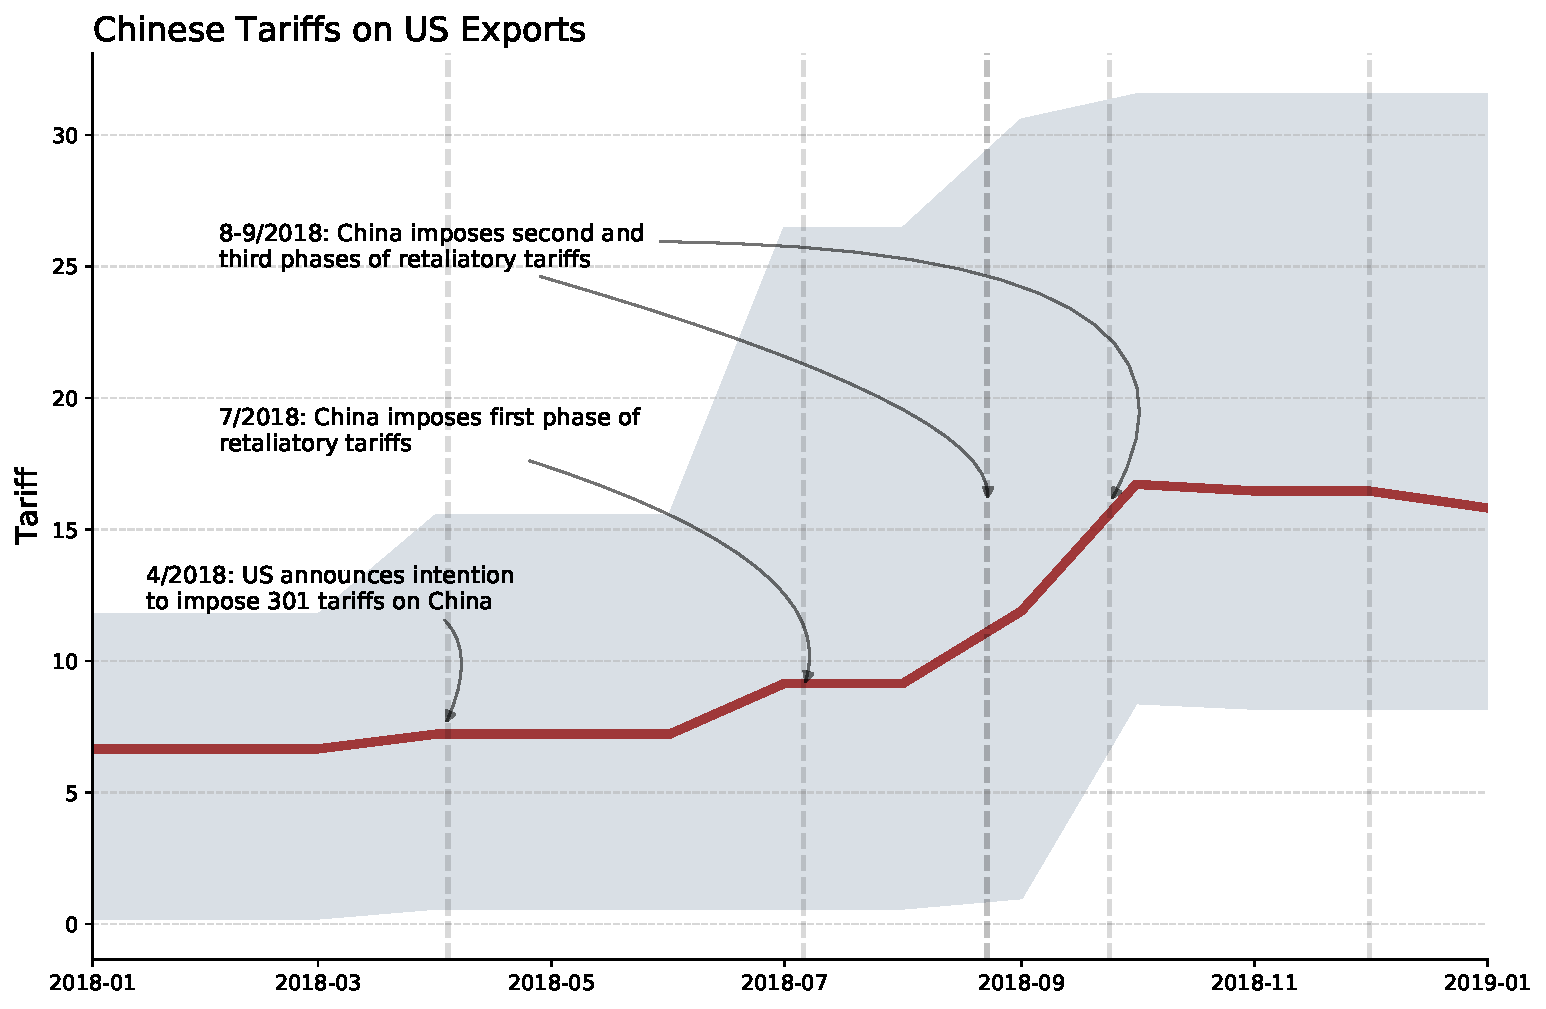
\includegraphics[scale = 0.6]{../figures/tariffs_time.pdf}}
\textbf{\caption{Chinese Tariffs on US Exports}\label{fig:tariffs}}
\end{figure}

Figure \ref{fig:tariffs} provides a high-level overview of the change in tariffs that US exporters faced. The dark red line reports the average tariff rate across all three-digit NAICS. The shaded band displays the upper 90then and lower 10th percentile in the distributions. Over this time period, tariffs have more than doubled. And coverage has been broad. Especially since the Phase 3 tariff lists, nearly all products to China faced some form of protection.

The trade flow data that I use is \href{https://www.census.gov/foreign-trade/data/index.html}{US Census Monthly International Trade Data}. This data set provides monthly totals of imports and exports, at varying HS-code levels, and by source and destination (and more). I focus on the period from January 2016 onward (so in 12 month differences the first observation starts in January 2017) As with the tariff data, I start at the HS6 level and then aggregate to three-digit NAICS codes. This is done for US exports to China and total US exports.

\subsection{Trade War Elasticities}

Table \ref{tb:war_rslts} reports the trade elasticity estimates. The first column reports the estimate from the specification in \ref{eq:trade_war}; the second column includes product-level fixed effects.

\begin{table}[!h]
\footnotesize
\refstepcounter{table}
\renewcommand{\arraystretch}{2.05}
\setlength {\tabcolsep}{3.5mm}
\begin{center}\label{tb:war_rslts}
\begin{tabular}{l c c}
\multicolumn{3}{c}{\normalsize \textbf{\ \ \ \ Table \ref{tb:war_rslts}: Estimates of Trade Elasticities \ \ \ \ }}\\
\hline
\hline
$\Delta \log\left(1+ \mbox{tr}_{ni,s,t} \right)$
& $\begin{array}{c}\textbf{-4.10}^{***} \vspace{-.45cm}\\ \scriptstyle \phantom{-}[ \ 1.31 \ ]\end{array}$
& $\begin{array}{c}\textbf{-3.22}^{***} \vspace{-.45cm}\\ \scriptstyle \phantom{-}[ \ 1.29 \ ]\end{array}$ \\
Time Effects            & Y & Y \\
County Fixed Effects    & N & Y \\
\hline
\# Observations &  900  \\
Time Period & \multicolumn{2}{l}{Jan 2017 - Jun 2019}\\
\hline
\end{tabular}
\parbox[c]{3.7in}{\vspace{.1cm}
{\footnotesize \textbf{Note:} Observations are weighted by 2016 level of trade. Standard errors are clustered at the product level and are reported in brackets.}}
\end{center}
\end{table}

You can not make this stuff up. What is amazing from this table is that the values are remarkably consistent with everything said above. Trade elasticities with values between three and four are the values most consistent with the trade response during the trade war. This is just like the price gap approach in Table \ref{tb:data_rslts} | elasticities with values between three and four. These are event consistent with elasticities from using tariffs and trade flow data in the cross-section.

These are slightly larger than what \citet{fajgelbaum2019return} are estimating. Not sure what the exact difference is. One issue is that they are jointly estimating a demand and supply curve, here I am not. My approach to seasonality is a bit different I think as well.

\section{What Next?}

First, I think some amount of success in the trade literature should be declared. From a theory standpoint, a lot of stuff is unified. From an empirical standpoint, I would say a clear message emerges about the value of the trade elasticity using very different approaches. With that said, I think there are some important aspects of measuring trade elasticities that need to be better understood:
\begin{itemize}
\item \textbf{More flexible substitution patterns.} I think the evidence from the trade war is calling out for this.

\item \textbf{Short-run vs. Long-run elasticities.} Obvious examples are \citet{ruhl2008}
\end{itemize}

\newpage

\small
\bibliography{micro_price_bibtex,big_bib_v6}

\end{document}
